\documentclass{standalone}
\usepackage{tikz}
\usetikzlibrary{patterns, positioning}

\begin{document}
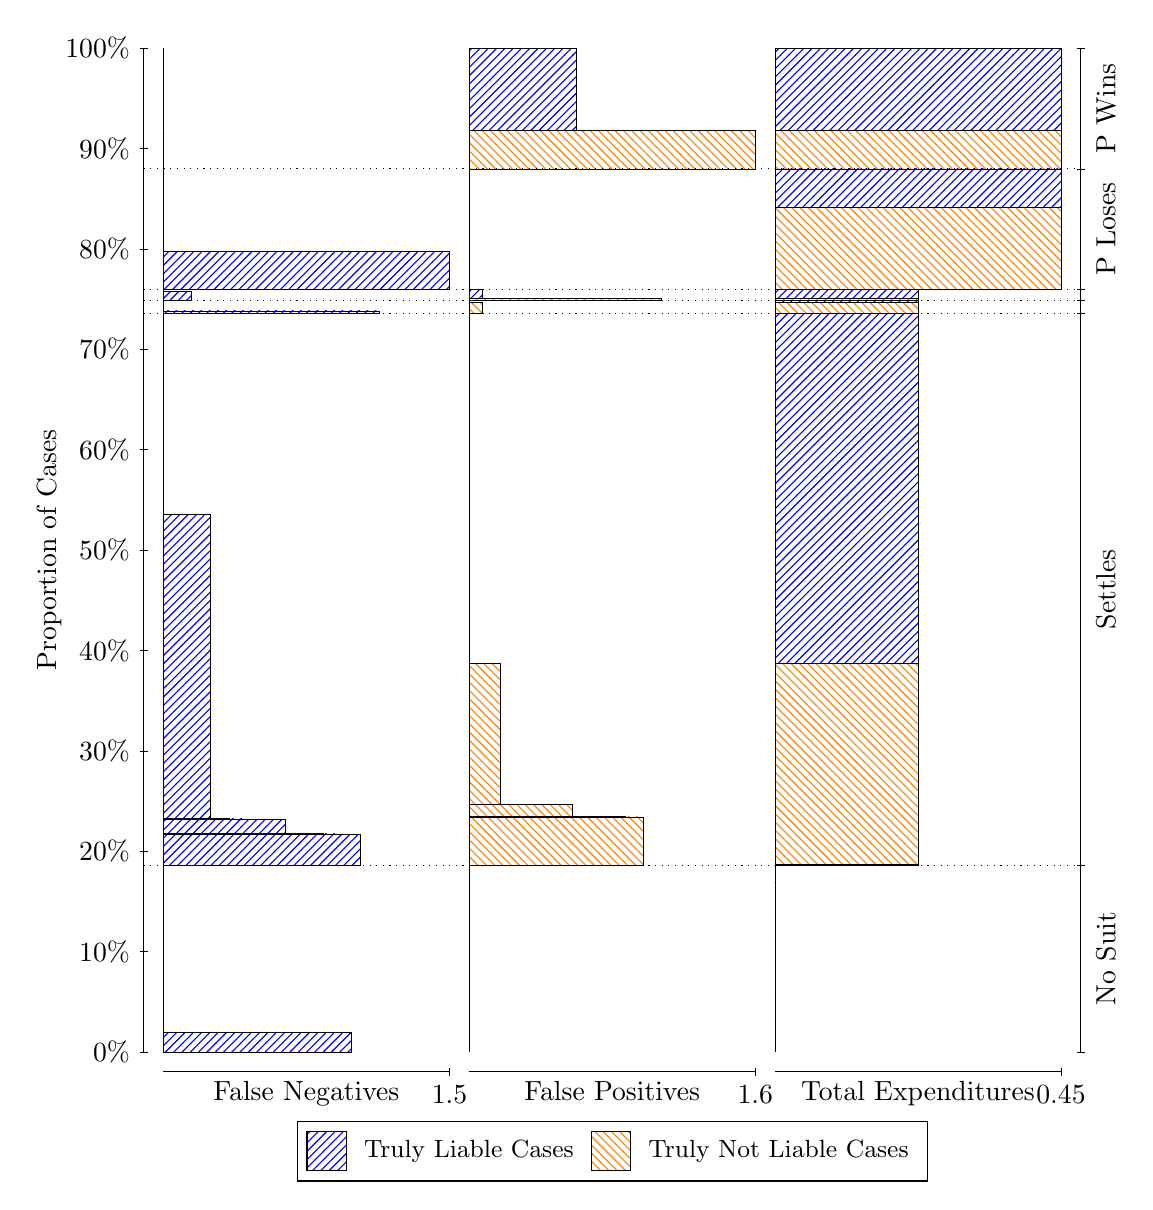
\begin{tikzpicture}
\draw[black, very thin] (1.5,1.75) -- (1.5,14.5);
\node[rotate=90, anchor=center] at (0.3, 8.125) {Proportion of Cases};
\draw[black, very thin] (1.45,1.75) -- (1.55,1.75);
\node[anchor=east] at (1.45, 1.75) {0\%};
\draw[black, very thin] (1.45,3.025) -- (1.55,3.025);
\node[anchor=east] at (1.45, 3.025) {10\%};
\draw[black, very thin] (1.45,4.3) -- (1.55,4.3);
\node[anchor=east] at (1.45, 4.3) {20\%};
\draw[black, very thin] (1.45,5.575) -- (1.55,5.575);
\node[anchor=east] at (1.45, 5.575) {30\%};
\draw[black, very thin] (1.45,6.85) -- (1.55,6.85);
\node[anchor=east] at (1.45, 6.85) {40\%};
\draw[black, very thin] (1.45,8.125) -- (1.55,8.125);
\node[anchor=east] at (1.45, 8.125) {50\%};
\draw[black, very thin] (1.45,9.4) -- (1.55,9.4);
\node[anchor=east] at (1.45, 9.4) {60\%};
\draw[black, very thin] (1.45,10.675) -- (1.55,10.675);
\node[anchor=east] at (1.45, 10.675) {70\%};
\draw[black, very thin] (1.45,11.95) -- (1.55,11.95);
\node[anchor=east] at (1.45, 11.95) {80\%};
\draw[black, very thin] (1.45,13.225) -- (1.55,13.225);
\node[anchor=east] at (1.45, 13.225) {90\%};
\draw[black, very thin] (1.45,14.5) -- (1.55,14.5);
\node[anchor=east] at (1.45, 14.5) {100\%};

\draw[black, very thin] (13.4,1.75) -- (13.4,14.5);
\draw[black, very thin] (13.35,1.75) -- (13.45,1.75);
\node[anchor=west] at (13.35, 1.75) {};
\draw[black, very thin] (13.35,4.1224) -- (13.45,4.1224);
\node[anchor=west] at (13.35, 4.1224) {};
\draw[black, very thin] (13.35,11.131) -- (13.45,11.131);
\node[anchor=west] at (13.35, 11.131) {};
\draw[black, very thin] (13.35,11.296) -- (13.45,11.296);
\node[anchor=west] at (13.35, 11.296) {};
\draw[black, very thin] (13.35,11.432) -- (13.45,11.432);
\node[anchor=west] at (13.35, 11.432) {};
\draw[black, very thin] (13.35,12.966) -- (13.45,12.966);
\node[anchor=west] at (13.35, 12.966) {};
\draw[black, very thin] (13.35,14.5) -- (13.45,14.5);
\node[anchor=west] at (13.35, 14.5) {};

\draw[black, very thin, pattern color=blue, pattern=north east lines] (1.75,1.75) rectangle (4.1325,1.9996);
\draw[black, very thin, pattern color=orange, pattern=north west lines] (1.75,1.9996) rectangle (1.75,4.1224);
\draw[black, very thin, pattern color=blue, pattern=north east lines] (1.75,4.1224) rectangle (4.2516,4.5178);
\draw[black, very thin, pattern color=blue, pattern=north east lines] (1.75,4.5178) rectangle (4.0134,4.5196);
\draw[black, very thin, pattern color=blue, pattern=north east lines] (1.75,4.5196) rectangle (3.7751,4.5215);
\draw[black, very thin, pattern color=blue, pattern=north east lines] (1.75,4.5215) rectangle (3.5369,4.5234);
\draw[black, very thin, pattern color=blue, pattern=north east lines] (1.75,4.5234) rectangle (3.2986,4.7035);
\draw[black, very thin, pattern color=blue, pattern=north east lines] (1.75,4.7035) rectangle (3.0604,4.7066);
\draw[black, very thin, pattern color=blue, pattern=north east lines] (1.75,4.7066) rectangle (2.8221,4.7099);
\draw[black, very thin, pattern color=blue, pattern=north east lines] (1.75,4.7099) rectangle (2.5839,4.7134);
\draw[black, very thin, pattern color=blue, pattern=north east lines] (1.75,4.7134) rectangle (2.3456,8.5727);
\draw[black, very thin, pattern color=orange, pattern=north west lines] (1.75,8.5727) rectangle (1.75,11.131);
\draw[black, very thin, pattern color=blue, pattern=north east lines] (1.75,11.131) rectangle (4.4899,11.161);
\draw[black, very thin, pattern color=orange, pattern=north west lines] (1.75,11.161) rectangle (1.75,11.296);
\draw[black, very thin, pattern color=blue, pattern=north east lines] (1.75,11.296) rectangle (2.1074,11.407);
\draw[black, very thin, pattern color=orange, pattern=north west lines] (1.75,11.407) rectangle (1.75,11.432);
\draw[black, very thin, pattern color=blue, pattern=north east lines] (1.75,11.432) rectangle (5.3833,11.918);
\draw[black, very thin, pattern color=orange, pattern=north west lines] (1.75,11.918) rectangle (1.75,12.966);
\draw[black, very thin, pattern color=orange, pattern=north west lines] (1.75,12.966) rectangle (1.75,13.452);
\draw[black, very thin, pattern color=blue, pattern=north east lines] (1.75,13.452) rectangle (1.75,14.5);
\draw[black, very thin, pattern color=orange, pattern=north west lines] (5.6333,1.75) rectangle (5.6333,3.8728);
\draw[black, very thin, pattern color=blue, pattern=north east lines] (5.6333,3.8728) rectangle (5.6333,4.1224);
\draw[black, very thin, pattern color=orange, pattern=north west lines] (5.6333,4.1224) rectangle (7.8474,4.7361);
\draw[black, very thin, pattern color=orange, pattern=north west lines] (5.6333,4.7361) rectangle (7.6203,4.739);
\draw[black, very thin, pattern color=orange, pattern=north west lines] (5.6333,4.739) rectangle (7.3932,4.7417);
\draw[black, very thin, pattern color=orange, pattern=north west lines] (5.6333,4.7417) rectangle (7.1661,4.7443);
\draw[black, very thin, pattern color=orange, pattern=north west lines] (5.6333,4.7443) rectangle (6.9391,4.8917);
\draw[black, very thin, pattern color=orange, pattern=north west lines] (5.6333,4.8917) rectangle (6.712,4.8917);
\draw[black, very thin, pattern color=orange, pattern=north west lines] (5.6333,4.8917) rectangle (6.712,4.8936);
\draw[black, very thin, pattern color=orange, pattern=north west lines] (5.6333,4.8936) rectangle (6.4849,4.8955);
\draw[black, very thin, pattern color=orange, pattern=north west lines] (5.6333,4.8955) rectangle (6.2578,4.8973);
\draw[black, very thin, pattern color=orange, pattern=north west lines] (5.6333,4.8973) rectangle (6.0307,6.6812);
\draw[black, very thin, pattern color=blue, pattern=north east lines] (5.6333,6.6812) rectangle (5.6333,11.131);
\draw[black, very thin, pattern color=orange, pattern=north west lines] (5.6333,11.131) rectangle (5.8036,11.266);
\draw[black, very thin, pattern color=blue, pattern=north east lines] (5.6333,11.266) rectangle (5.6333,11.296);
\draw[black, very thin, pattern color=orange, pattern=north west lines] (5.6333,11.296) rectangle (8.0745,11.321);
\draw[black, very thin, pattern color=blue, pattern=north east lines] (5.6333,11.321) rectangle (5.8036,11.432);
\draw[black, very thin, pattern color=orange, pattern=north west lines] (5.6333,11.432) rectangle (5.6333,12.48);
\draw[black, very thin, pattern color=blue, pattern=north east lines] (5.6333,12.48) rectangle (5.6333,12.966);
\draw[black, very thin, pattern color=orange, pattern=north west lines] (5.6333,12.966) rectangle (9.2667,13.452);
\draw[black, very thin, pattern color=blue, pattern=north east lines] (5.6333,13.452) rectangle (6.9958,14.5);
\draw[black, very thin, pattern color=orange, pattern=north west lines] (9.5167,1.75) rectangle (9.5167,3.8728);
\draw[black, very thin, pattern color=blue, pattern=north east lines] (9.5167,3.8728) rectangle (9.5167,4.1224);
\draw[black, very thin, pattern color=orange, pattern=north west lines] (9.5167,4.1224) rectangle (11.333,4.1224);
\draw[black, very thin, pattern color=blue, pattern=north east lines] (9.5167,4.1224) rectangle (11.333,4.1225);
\draw[black, very thin, pattern color=orange, pattern=north west lines] (9.5167,4.1225) rectangle (11.333,4.128);
\draw[black, very thin, pattern color=blue, pattern=north east lines] (9.5167,4.128) rectangle (11.333,4.1336);
\draw[black, very thin, pattern color=orange, pattern=north west lines] (9.5167,4.1336) rectangle (11.333,6.6868);
\draw[black, very thin, pattern color=blue, pattern=north east lines] (9.5167,6.6868) rectangle (11.333,11.131);
\draw[black, very thin, pattern color=orange, pattern=north west lines] (9.5167,11.131) rectangle (11.333,11.266);
\draw[black, very thin, pattern color=blue, pattern=north east lines] (9.5167,11.266) rectangle (11.333,11.296);
\draw[black, very thin, pattern color=orange, pattern=north west lines] (9.5167,11.296) rectangle (11.333,11.321);
\draw[black, very thin, pattern color=blue, pattern=north east lines] (9.5167,11.321) rectangle (11.333,11.432);
\draw[black, very thin, pattern color=orange, pattern=north west lines] (9.5167,11.432) rectangle (13.15,12.48);
\draw[black, very thin, pattern color=blue, pattern=north east lines] (9.5167,12.48) rectangle (13.15,12.966);
\draw[black, very thin, pattern color=orange, pattern=north west lines] (9.5167,12.966) rectangle (13.15,13.452);
\draw[black, very thin, pattern color=blue, pattern=north east lines] (9.5167,13.452) rectangle (13.15,14.5);
\draw[black, dotted] (1.5,4.1224) -- (13.4,4.1224);
\draw[black, dotted] (1.5,11.131) -- (13.4,11.131);
\draw[black, dotted] (1.5,11.296) -- (13.4,11.296);
\draw[black, dotted] (1.5,11.432) -- (13.4,11.432);
\draw[black, dotted] (1.5,12.966) -- (13.4,12.966);
\draw[black, very thin] (1.75,1.5) -- (5.3833,1.5);
\node[anchor=north] at (3.5667, 1.5) {False Negatives};
\draw[black, very thin] (5.3833,1.45) -- (5.3833,1.55);
\node[anchor=north] at (5.3833, 1.45) {1.5};

\draw[black, very thin] (5.6333,1.5) -- (9.2667,1.5);
\node[anchor=north] at (7.45, 1.5) {False Positives};
\draw[black, very thin] (9.2667,1.45) -- (9.2667,1.55);
\node[anchor=north] at (9.2667, 1.45) {1.6};

\draw[black, very thin] (9.5167,1.5) -- (13.15,1.5);
\node[anchor=north] at (11.333, 1.5) {Total Expenditures};
\draw[black, very thin] (13.15,1.45) -- (13.15,1.55);
\node[anchor=north] at (13.15, 1.45) {0.45};

\node[black, centered, rotate=90] at (13.72, 2.9362) {No Suit};
\node[black, centered, rotate=90] at (13.72, 7.6269) {Settles};


\node[black, centered, rotate=90] at (13.72, 12.199) {P Loses};
\node[black, centered, rotate=90] at (13.72, 13.733) {P Wins};

\draw (7.449999999999999,1.5) node[draw=none] (baseCoordinate) {};
\begin{scope}[align=center]
        \matrix[scale=0.5, draw=black, below=0.5cm of baseCoordinate, nodes={draw}, column sep=0.1cm]{
            \node[rectangle, draw, minimum width=0.5cm, minimum height=0.5cm, pattern=north east lines, pattern color=blue] {}; &
            \node[draw=none, font=\small] (B) {Truly Liable Cases}; &
            \node[rectangle, draw, minimum width=0.5cm, minimum height=0.5cm, pattern=north west lines, pattern color=orange] {}; &
            \node[draw=none, font=\small] (B) {Truly Not Liable Cases}; \\
            };
\end{scope}

\end{tikzpicture}
\end{document}